%% Los cap'itulos inician con \chapter{T'itulo}, estos aparecen numerados y
%% se incluyen en el 'indice general.
%%
%% Recuerda que aqu'i ya puedes escribir acentos como: 'a, 'e, 'i, etc.
%% La letra n con tilde es: 'n.

\chapter{Results}

The following section is dedicated to expose the different results obtained after using the developed \textit{Measure System}. With the results obtained we will decide if it is possible or not to use this system for future studies.\\

Also, it will be compared the different results obtained with the ideal model used in this study. In this section it will be explained the different studied cases used to test system. With all these studied cases it will be possible to get all the information needed to decide if the system is affordable or not.

\section{Studied cases}

The purpose of this project is to find a solution that can be used for studying the properties of materials that formed part of floors. This solution should obtain accurate measures, it should be use to manage and it should be affordable. All this information was described before with more details.\\

In this section it will be commented the different use cases used to test the system. These use cases allow us to determine if the project could be used or not. It is important to say that it is necessary to test this system with different values using as reference the actual system used.\\

Another important thing is that we need to know if the sensors used don not have variations in their accuracy when the media has different values of humidity.\\

There are lot of factor which will influence in the results we will get. The results could change if we consider the following factors:

\begin{itemize}

\item Inclination of the substratum. The humidity will change depending on how tilted is the substratum. Depending on the area we are analyzing, the measures could change.

\item Current state of the sensors. The sensors could be damaged if they are connected for a long time. It is not the same to use a new sensor to use a degraded sensor which was connected to the system since months.

\item Type of substratum used in the study. Depending on the substratum we are using in the study, the results could change getting different values. Not all the substrates have the same period of drying. It is an important topic to consider in the study.

\item Environmental temperature. If there changes in the environmental temperatures the results can vary. If the environmental temperature is constant the results will follow the ideal model used for the study.

\end{itemize}

The values used for testing the system are described in the following points.

\begin{itemize}

\item Values registered with \%

\item Values registered with \%

\item Values registered with \%

\item Values registered with \%

\end{itemize}

\section{Analysis of the results obtained}

After studying the different use cases that could be presented in the system, it is necessary to study the results obtained and decide if the system can be used for future studies of materials.\\

For doing this study, it is necessary to have a representation of the information. This representation has to be done with graphs that can allow us to determine if the measures are reliable or not.\\

The results obtained have to be compared with results obtained by accurate systems. The results obtained by other systems have to present in graphs to. If we want to do this comparison, it is necessary to build our graphs with the information monitored by the system. These graphs will be done using Microsoft Excel. For building these graphs, it is necessary to select the results that we want to represent selecting the dates that correspond to the measured obtained in the use cases.\\

After doing it, we select the graph where we want to represent the information. After doing it, we build the graph that we want to compare. If we have previous studies we can compare the results obtained with new ones.\\

%METER AQUI GRÁFICAS DEL SISTEMA NUESTRO
The following picture represents the ideal dried graphic used as reference. This graph represents how the vales can change in an ideal study.

\begin{figure}[H]
\begin{centering}
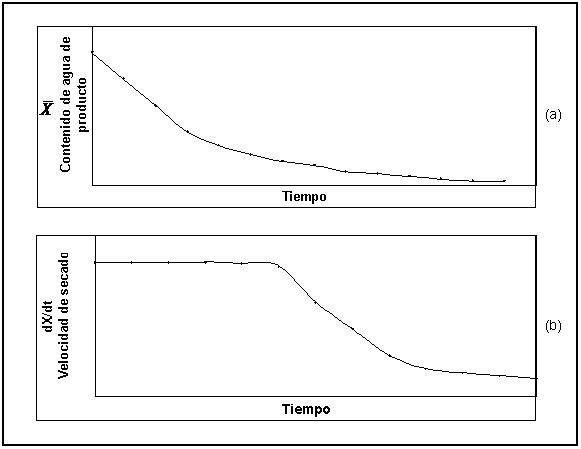
\includegraphics[scale=0.6]{IMGS/secado_ideal.jpg}
\caption{Ideal dried graphic \label{Ideal dried graphic}}
\end{centering}
\end{figure}

As it is possible to see, this picture allows us to know how is the evolution of the measure when the time changes.\\

In the following picture, it is showed the results obtained after using the developed system.

\begin{figure}[H]
\begin{centering}
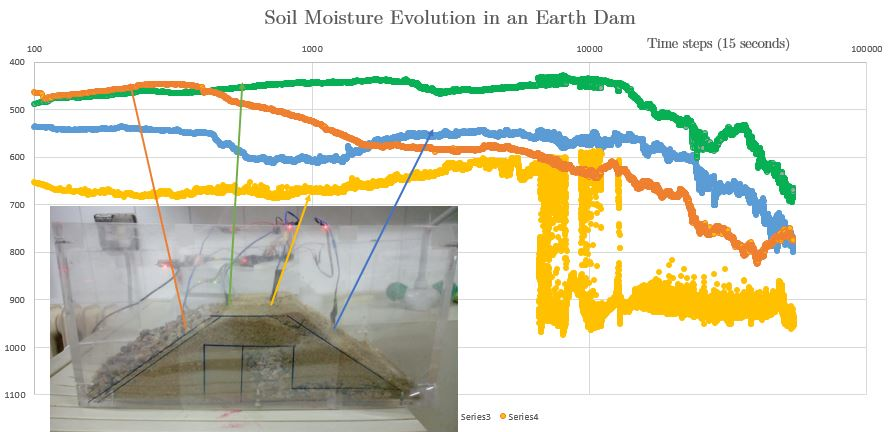
\includegraphics[scale=0.6]{IMGS/results_measures.jpeg}
\caption{Soil Moisture Evolution in an Earth Dam \label{Soil Moisture Evolution in an Earth Dam}}
\end{centering}
\end{figure} 

It is possible to see that the represented graph is similar to the one used as model of study. It is important to consider that the time interval used is minor that the one represented in the ideal model.\\

With both graphs, we can determine that the results obtained in this study are completely valid. It is possible to  say that the system developed could be applied to future studies. We can see that the curves of the drying process are really similar to the graphs obtained by reliable systems.\\

\newpage


